% Options for packages loaded elsewhere
\PassOptionsToPackage{unicode}{hyperref}
\PassOptionsToPackage{hyphens}{url}
\PassOptionsToPackage{dvipsnames,svgnames,x11names}{xcolor}
%
\documentclass[
  12pt,
]{article}
\usepackage{amsmath,amssymb}
\usepackage{lmodern}
\usepackage{iftex}
\ifPDFTeX
  \usepackage[T1]{fontenc}
  \usepackage[utf8]{inputenc}
  \usepackage{textcomp} % provide euro and other symbols
\else % if luatex or xetex
  \usepackage{unicode-math}
  \defaultfontfeatures{Scale=MatchLowercase}
  \defaultfontfeatures[\rmfamily]{Ligatures=TeX,Scale=1}
\fi
% Use upquote if available, for straight quotes in verbatim environments
\IfFileExists{upquote.sty}{\usepackage{upquote}}{}
\IfFileExists{microtype.sty}{% use microtype if available
  \usepackage[]{microtype}
  \UseMicrotypeSet[protrusion]{basicmath} % disable protrusion for tt fonts
}{}
\makeatletter
\@ifundefined{KOMAClassName}{% if non-KOMA class
  \IfFileExists{parskip.sty}{%
    \usepackage{parskip}
  }{% else
    \setlength{\parindent}{0pt}
    \setlength{\parskip}{6pt plus 2pt minus 1pt}}
}{% if KOMA class
  \KOMAoptions{parskip=half}}
\makeatother
\usepackage{xcolor}
\usepackage[margin=1in]{geometry}
\usepackage{longtable,booktabs,array}
\usepackage{calc} % for calculating minipage widths
% Correct order of tables after \paragraph or \subparagraph
\usepackage{etoolbox}
\makeatletter
\patchcmd\longtable{\par}{\if@noskipsec\mbox{}\fi\par}{}{}
\makeatother
% Allow footnotes in longtable head/foot
\IfFileExists{footnotehyper.sty}{\usepackage{footnotehyper}}{\usepackage{footnote}}
\makesavenoteenv{longtable}
\usepackage{graphicx}
\makeatletter
\def\maxwidth{\ifdim\Gin@nat@width>\linewidth\linewidth\else\Gin@nat@width\fi}
\def\maxheight{\ifdim\Gin@nat@height>\textheight\textheight\else\Gin@nat@height\fi}
\makeatother
% Scale images if necessary, so that they will not overflow the page
% margins by default, and it is still possible to overwrite the defaults
% using explicit options in \includegraphics[width, height, ...]{}
\setkeys{Gin}{width=\maxwidth,height=\maxheight,keepaspectratio}
% Set default figure placement to htbp
\makeatletter
\def\fps@figure{htbp}
\makeatother
\setlength{\emergencystretch}{3em} % prevent overfull lines
\providecommand{\tightlist}{%
  \setlength{\itemsep}{0pt}\setlength{\parskip}{0pt}}
\setcounter{secnumdepth}{5}
\newlength{\cslhangindent}
\setlength{\cslhangindent}{1.5em}
\newlength{\csllabelwidth}
\setlength{\csllabelwidth}{3em}
\newlength{\cslentryspacingunit} % times entry-spacing
\setlength{\cslentryspacingunit}{\parskip}
\newenvironment{CSLReferences}[2] % #1 hanging-ident, #2 entry spacing
 {% don't indent paragraphs
  \setlength{\parindent}{0pt}
  % turn on hanging indent if param 1 is 1
  \ifodd #1
  \let\oldpar\par
  \def\par{\hangindent=\cslhangindent\oldpar}
  \fi
  % set entry spacing
  \setlength{\parskip}{#2\cslentryspacingunit}
 }%
 {}
\usepackage{calc}
\newcommand{\CSLBlock}[1]{#1\hfill\break}
\newcommand{\CSLLeftMargin}[1]{\parbox[t]{\csllabelwidth}{#1}}
\newcommand{\CSLRightInline}[1]{\parbox[t]{\linewidth - \csllabelwidth}{#1}\break}
\newcommand{\CSLIndent}[1]{\hspace{\cslhangindent}#1}
\usepackage{setspace} % line spacing
\usepackage{geometry} % margins, etc
\geometry{margin=2.5cm}
\usepackage[nottoc]{tocbibind} % lof and lot in toc
\usepackage{caption} % captions formatting
\captionsetup{justification   = raggedright,
              singlelinecheck = false,
              format = hang,
              labelfont = bf}
\usepackage{tocloft} % lof and lot editing
\renewcommand{\cftfigfont}{Figure }
\renewcommand{\cfttabfont}{Table }
\expandafter\def\expandafter\quote\expandafter{\quote\singlespacing} %single spacing in quotes

\AtBeginDocument{\let\maketitle\relax}

\usepackage{fontspec}
\setmainfont{Times New Roman}

\usepackage{dcolumn}

% Avoid weird line and word breaks
\tolerance = 1
\emergencystretch = \maxdimen
\hyphenpenalty = 10000
\hbadness = 10000
\usepackage{booktabs}
\usepackage{longtable}
\usepackage{array}
\usepackage{multirow}
\usepackage{wrapfig}
\usepackage{float}
\usepackage{colortbl}
\usepackage{pdflscape}
\usepackage{tabu}
\usepackage{threeparttable}
\usepackage{threeparttablex}
\usepackage[normalem]{ulem}
\usepackage{makecell}
\usepackage{xcolor}
\ifLuaTeX
  \usepackage{selnolig}  % disable illegal ligatures
\fi
\IfFileExists{bookmark.sty}{\usepackage{bookmark}}{\usepackage{hyperref}}
\IfFileExists{xurl.sty}{\usepackage{xurl}}{} % add URL line breaks if available
\urlstyle{same} % disable monospaced font for URLs
\hypersetup{
  pdftitle={Focus on the content},
  pdfauthor={Antonio Fidalgo and Simão Nogueira},
  colorlinks=true,
  linkcolor={black},
  filecolor={Maroon},
  citecolor={Blue},
  urlcolor={Blue},
  pdfcreator={LaTeX via pandoc}}

\title{Focus on the content}
\usepackage{etoolbox}
\makeatletter
\providecommand{\subtitle}[1]{% add subtitle to \maketitle
  \apptocmd{\@title}{\par {\large #1 \par}}{}{}
}
\makeatother
\subtitle{A Rmd template for writing a Master's dissertation at CLSBE}
\author{Antonio Fidalgo and Simão Nogueira}
\date{October 6, 2022}

\begin{document}
\maketitle

\pagenumbering{gobble}

\begin{figure}

{\centering 
\includegraphics[width=0.66\linewidth]{figures/logo} 

}

\end{figure}

\begin{centering}
\vfill
\begin{spacing}{1.0}
\parbox{35em}{\centering\Huge\bf  Focus on the content} \\
\vspace{\baselineskip}
\parbox{35em}{\centering\LARGE  A Rmd template for writing a Master's dissertation at CLSBE }
\end{spacing}
\vfill 
{\LARGE\bf Antonio Fidalgo and Simão Nogueira }
\vfill 
\parbox{35em}{\centering\Large Dissertation written under the supervision of Prof. R2D2.} 
\vfill 
\parbox{35em}{\centering\Large Dissertation submitted in partial fulfilment of requirements for the MSc in Reproducible Business, at the Universidade Católica Portuguesa.\\% 
\vspace{\baselineskip}
October 6, 2022}

\end{centering}
\clearpage
\pagenumbering{roman}

\pagenumbering{gobble}
\vspace*{\fill}

\begin{flushright}
To our students.
\end{flushright}

\vspace*{\fill}

\clearpage
\pagenumbering{roman}

\hypertarget{acknowledgments}{%
\section*{Acknowledgments}\label{acknowledgments}}
\addcontentsline{toc}{section}{Acknowledgments}

We drew a great deal of inspiration from books and papers such as Xie (\protect\hyperlink{ref-Xie_2015}{2015}) and Wickham (\protect\hyperlink{ref-Wickham_2010}{2010}). We deeply thank their authors, Yihui Xie and Hadley Wickham, for these fantastic contributions.

The usual disclaimer applies.

\clearpage

\hypertarget{abstract}{%
\section*{Abstract}\label{abstract}}
\addcontentsline{toc}{section}{Abstract}

\textbf{Title:} Focus on the content. A Rmd template for writing a Master's dissertation at CLSBE\\
\textbf{Author:} Antonio Fidalgo and Simão Nogueira\\
\textbf{Keywords:} Reproducible research; Dynamic document; Master thesis.

\vspace{3\baselineskip}

Abstract here\ldots{}

\clearpage

\hypertarget{resumo}{%
\section*{Resumo}\label{resumo}}
\addcontentsline{toc}{section}{Resumo}

\textbf{Title:} Focus on the content. A Rmd template for writing a Master's dissertation at CLSBE\\
\textbf{Author:} Antonio Fidalgo and Simão Nogueira\\
\textbf{Palavras-chave:} Investigação reproduzível; Documento Dinâmico; Tese de Mestrado.

\vspace{3\baselineskip}

Resumo aqui\ldots{}

\clearpage\tableofcontents
\clearpage\listoffigures
\clearpage\listoftables

\clearpage

\hypertarget{list-of-acronyms-and-abbreviations}{%
\section*{List of Acronyms and Abbreviations}\label{list-of-acronyms-and-abbreviations}}
\addcontentsline{toc}{section}{List of Acronyms and Abbreviations}

\begin{table}[H]
\begin{tabular}{>{\raggedright\arraybackslash}p{2cm}l}
\toprule
\textbf{Acronym/ Abbrev.} & \textbf{Definition}\\
\midrule
\cellcolor{gray!6}{NUTS} & \cellcolor{gray!6}{Nomenclature of Territorial Units for Statistics}\\
R2D2 & Reproducible Research \& Dynamic Document\\
\bottomrule
\end{tabular}
\end{table}

\clearpage
\pagenumbering{arabic}\setcounter{page}{1}
\onehalfspacing

\hypertarget{introduction}{%
\section{Introduction}\label{introduction}}

Since time immemorial\ldots{} really?

\clearpage

\hypertarget{conclusion}{%
\section{Conclusion}\label{conclusion}}

\begin{figure}

{\centering 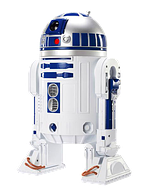
\includegraphics[width=0.2\linewidth]{figures/r2d2} 

}

\caption{My supervisor.}\label{fig:r2d2pic}
\end{figure}

\clearpage

\hypertarget{references}{%
\section*{References}\label{references}}
\addcontentsline{toc}{section}{References}

\hypertarget{refs}{}
\begin{CSLReferences}{1}{0}
\leavevmode\vadjust pre{\hypertarget{ref-rmdtemplate}{}}%
Fidalgo, Antonio, and Simão Nogueira. 2022. {``Focus on the Content: A Rmd Template for Writing a Master's Dissertation at CLSBE.''}

\leavevmode\vadjust pre{\hypertarget{ref-Wickham_2010}{}}%
Wickham, Hadley. 2010. {``A Layered Grammar of Graphics.''} \emph{Journal of Computational and Graphical Statistics} 19 (1): 3--28.

\leavevmode\vadjust pre{\hypertarget{ref-Xie_2015}{}}%
Xie, Yihui. 2015. \emph{Dynamic Documents with {R} and Knitr}. 2nd ed. Boca Raton, Florida: Chapman; Hall/CRC.

\end{CSLReferences}

\clearpage

\appendix

\hypertarget{appendix}{%
\section{Appendix}\label{appendix}}

\end{document}
